\documentclass{sig-alternate}

\usepackage{times}

\usepackage{url}
\urlstyle{it}
\usepackage{graphicx}
\usepackage{graphics}
\usepackage{subfig}
\usepackage{longtable}
\usepackage{array}
\usepackage{multirow}
\usepackage{textcomp}
\usepackage{framed,color}
% Paragraphs
\newcommand{\spara}[1]{\smallskip\noindent{\bf #1}}
\newcommand{\mpara}[1]{\medskip\noindent{\bf #1}}
\newcommand{\para}[1]{\noindent{\bf #1}}

\clubpenalty=10000
\widowpenalty=10000

%% Define a new 'leo' style for the package that will use a smaller font.
\makeatletter
\def\url@leostyle{%
  
\@ifundefined{selectfont}{\def\UrlFont{\sf}}{\def\UrlFont{\scriptsize\ttfamily}}}
\makeatother
%% Now actually use the newly defined style.
\urlstyle{leo}




\begin{document}
%\conferenceinfo{WISDOM'13,}{August 11 2013, Chicago, IL, USA}
 

%\crdata{978-1-4503-2332-1/13/08}
%\CopyrightYear{2013}

% Place holder, can be changed if wanted
\title{ A time-series classification model for Twitter opinion lexicon expansion}

% Propose this new titlte
% Supervised opinion lexicon expansion from automatically labelled tweets

\numberofauthors{3}
\author{
% You can go ahead and credit any number of authors here,
% e.g. one 'row of three' or two rows (consisting of one row of three
% and a second row of one, two or three).
%
% The command \alignauthor (no curly braces needed) should
% precede each author name, affiliation/snail-mail address and
% e-mail address. Additionally, tag each line of
% affiliation/address with \affaddr, and tag the
% e-mail address with \email.
%
% 1st. author
\alignauthor
Felipe Bravo-Marquez\\
	\affaddr{Department of Computer Science, University of Waikato, New Zealand}\\
	\email{\scriptsize{fjb11@students.waikato.ac.nz}}
\alignauthor Eibe Frank\\
       \affaddr{Department of Computer Science, University of Waikato, New Zealand}\\
       \email{eibe@waikato.ac.nz}
\alignauthor Bernhard Pfahringer\\
       \affaddr{Department of Computer Science, University of Waikato, New Zealand}\\
       \email{bernhard@waikato.ac.nz}
}



\maketitle

\begin{abstract}
Opinion lexicons, which are lists of terms labelled by sentiment, are widely used resources to support automatic sentiment analysis of textual passages. However, these resources exhibit important limitations when applied to social media messages such as tweets (posts in Twitter), because they are unable to capture the diversity of informal expressions commonly found in this type of media. In this article, we propose a process to automatically categorise Twitter words into three sentiment classes: positive, neutral, and negative. The expansion is done through a supervised learning process in which word-level attributes are calculated from a multi-dimensional time-series, and a seed lexicon of labelled words is used as the training dataset. The time-series are extracted from a temporal collection of automatically labelled tweets representing the relationship between the word and the sentiment expressed in the tweets where it occurs. Our experimental results show that our method outperforms the word-level sentiment classification performance obtained by semantic orientation, a well known state-of-the-art measure for establishing world-level sentiment. Additionally, we show that our expanded lexicon produces significant improvements when used for message-level polarity classification of tweets.


\end{abstract}

\category{I.2.7.7}{Artificial Intelligence}{Natural Language Processing}[Text Analysis]

\terms{Experimentation, Measurement}

\keywords{Lexicon Expansion, Sentiment Analysis, Twitter}


\section{Introduction}\label{sec:intro}

Several sentiment analysis methods rely on lexical resources for evaluating the sentiment of a text passage, in particular they often rely on an opinion lexicon. An opinion or sentiment lexicon is a dictionary of opinion words with their corresponding sentiment values. Lexicons can be used to compute the polarity of a message by aggregating the orientation values of the opinion words found in the document \cite{Wiebe2000}. They have also proven to be useful when used to extract features in supervised classification schemes~\cite{jiang2011target, kouloumpis2011twitter,Zirn20011}. 

Social media platforms and, in particular, microblogging services such as \textbf{Twitter}\footnote{\url{http://www.twitter.com}}, are increasingly being adopted by people to access and publish information about a great variety of topics. Sentiment analysis applied to social media posts has received an increasing interest due to its importance in a wide range of fields such as business, sports, and politics. However, the language used in Twitter provides substantial challenges for sentiment analysis. The words used in this platform include many abbreviations, acronyms, and misspelled words which are not observed in traditional media and are not covered by most popular lexicons such as OpinionFinder \cite{Wilson2005}, SentiWordnet \cite{esuli2006}, and the Harvard General Inquirer \cite{stone66}. The diversity and sparseness of these informal words make the manually creation of a Twitter-oriented opinion lexicon a time-consuming task.

% Words can be positive, negative, or neutral depending on the context

In this article we propose a supervised framework for opinion lexicon expansion for the language used in Twitter.  Taking SentiWordnet as inspiration, each word in our expanded lexicon has a probability distribution, describing how positive, negative, and neutral it is.  Additionally, all the entries of the lexicon are associated with a corresponding part-of-speech tag. We believe that estimating the sentiment distribution of POS-tagged words according the three opinion-related properties may be useful for developing Twitter-specific sentiment applications due to the following reasons:

\begin{enumerate}
%\item There are some words in which its opinion-related properties can change from one domain to another, e.g., the word \emph{small} is positive when referring to a queue in a bank but negative when referring to a hotel room. These type of words could be represented by having probabilities greater than zero for both positive and negative classes.
\item A word can present certain levels of intensity \cite{ThelwallBP12} for a specific sentiment category e.g., the word \emph{awesome} is more positive than the word \emph{adequate}. The estimated probabilities could be used to represent these levels of intensities.

\item  The neutral score provided by the lexicon could be useful for discarding non-opinion words in text-level polarity classification tasks. This can be easily done  taking the class with the maximum probability and discarding words classified as neutral. On the other hand, unsupervised lexicon expansion techniques such as semantic orientation \cite{Turney2002} provide a single numerical score for each word. It is no clear how to find a threshold for using this score in neutrality detection. 

\item   Homographs, which are  words that share the same spelling but have different meanings, should  have different lexicon entries for each different meaning. By relying on POS-tagged words, homographs with different POS-tags will be disambiguated \cite{wilks1998grammar}. For instance, the word \emph{apple}  will receive different sentiment scores when used to refer to a common noun (a fruit) or a proper noun (a company). 

\end{enumerate}


The proposed methodology takes a collection of tweets labelled according to their polarity to establish a polarity-related time-series for each POS-tagged word in the tweets and uses features extracted from this time-series in relation with the labels provided by a seed lexicon to train a word-level sentiment classifier. The seed lexicon is taken from the union of different hand-made lexicons after discarding all polarity clashes from the intersection. Furthermore, the tweets from the collection are labelled using a semi-supervised heuristics to avoid the expensive costs of data annotation called \emph{emoticon-based annotation}. In this approach, only tweets having positive or negative emoticons are considered and labelled according to the polarity indicated by the emoticon. This idea has been widely used before to train message-level sentiment classifiers \cite{bifet2010, go2010, pak2010twitter}.

%In the second approach, the tweets are classified into classes positive, negative and neutral using two sentiment analysis tools: \emph{SentiStrength}\footnote{\url{http://sentistrength.wlv.ac.uk/}} and \emph{Sentiment140}\footnote{\url{http://www.sentiment140.com/}}. Afterwards, all tweets in which both methods disagree are discarded. 


Our word-level time-series are computed from two different criteria: Semantic Orientation (SO) \cite{Turney2002}, which is based on the mutual information between word and sentiment class, and Stochastic Gradient Descent (SGD) score, which learns a linear relationship between word and sentiment class.

The proposed procedure can be summarised in the following steps:

\begin{enumerate}
\item Collect tweets from the domain and the time period for which the lexicon needs to be expanded. 
\item Label the collection with sentiment classes in an automatic way.
\item Tag all the words using a part-of-speech tagger.
\item Calculate word-level time-series for all tagged words and extract sentiment features from them.
\item Label the sentiment of the words that match an existing hand-made polarity lexicon.
\item Train a word-level classifier using the word-level features and the words labels from the seed lexicon.
\item Use the trained classifier to estimate the polarity distribution of the remaining unlabelled words.
\end{enumerate}
 
%Briefly explain the experiments 
As will be discussed in Section~\ref{sec:related}, the automatic expansion of Twitter  opinion words has been studied before \cite{avaya2013,Mohammad2013,Zhou2014}. In all these works, the expansion was conducted using semantic orientation, which is an unsupervised measure.  
To the best of our knowledge, this is the first article in which the lexicon expansion of Twitter opinion words is studied and evaluated using POS disambiguation and supervised learning. Additionally, this is the first study in which scores for positive, negative, and neutral opinion-related properties are provided for Twitter-specific expressions.


%It is important to remark that a supervised word labelling approach based on a seed lexicon provides flexibility in determining the desired nature of the polarity label of the expanded words. For instance, we can compute a categorical label through classification or a numerical score through regression. On the other hand, when the lexicon is created from  unsupervised measures such as semantic orientation is it not clear how to transform these values into the desired labels.  


%This is the first study comparing two different mechanisms for automatic labelling tweets for lexicon expansion (Emoticon Labels and Consensus of methods).

%This is the first study combining the semantic orientation measure with POS tags (POS tags were used before as filters to discard words from POS that are unlikely to express an opinion). This is the first study in Twitter lexicon expansion including the detection of neutral words. This is the first study in which semantic orientation is compared and combined with SGD scores. 
 
We test our approach on two collections of automated labelled tweets. Our results indicate that our supervised framework outperforms the classification accuracy obtained by  semantic orientation when the detection of neutral words is included. We also evaluate the usefulness of the expanded lexicon for message-level polarity classification of tweets, showing significant improvements in performance.   
 
This article in organised as follows. In Section~\ref{sec:related} we provide a review of existing work in opinion lexicon expansion. In Section~\ref{sec:seed_lex} we describe the seed lexicon used to label the words for the training set. In Section~\ref{sec:tweetlab} we explain the mechanisms studied to automatically create collections of labelled tweets.
 The creation of our word-level time-series is described in Section~\ref{sec:feat}, together with the features used for training the classifier. In Section~\ref{sec:lex_expand} we present the experiments we conducted to evaluate the proposed approach and we also discuss the obtained results. The main findings and conclusions are discussed in Section~\ref{sec:conc}.

\section{Related Work}\label{sec:related}
There are basically two type of resources which can be exploited for lexicon expansion: a  thesaurus and a corpus of documents. The simplest approach using a thesaurus such as WordNet\footnote{\url{http://wordnet.princeton.edu/}} is to expand a seed lexicon of labelled opinion words using synonyms and antonyms from the lexical relations provided by the thesaurus 
\cite{Liu2004,Kim2004}. The hypothesis behind this approach is that synonyms may have the same polarity and antonyms may have the opposite. This process is normally iterated several times.
In \cite{kamps2004} a graph was created using WordNet adjectives as vertices and the synonym relation as edges. The orientation of a term is determined by its relative distance from two seed terms \emph{good} and \emph{bad}. In \cite{Esuli2005} a supervised classifier was trained using a seed of labelled words which was obtained through synonyms and antonyms expansion. For each word, a vector space model is created from the definition or \emph{gloss} provided by the WordNet dictionary. This representation is used to train a word-level classifier that is used for lexicon expansion. An equivalent approach was applied later to create SentiWordnet\footnote{\url{http://sentiwordnet.isti.cnr.it/}} in \cite{esuli2006, Baccianella2010}. In SentiWordNet each WordNet \emph{synset} or group of synonyms is  annotated into classes positive, negative and neutral in the range $[0,1]$.    

A limitation of thesaurus-based approaches is their inability to capture domain dependent words. On the other hand, corpus-based approaches exploit syntactic or co-occurrence patterns to expand the lexicon to the words found within a collection of documents. 
In \cite{Hatziva1997}, the proposed method starts with a set of adjectives whose polarity is known and then discovers the polarities of new adjectives using some linguistic patterns from a corpus of documents. The authors show, using log-linear regression, that conjunctions between adjectives provide indirect information about the orientation. For example, adjectives connected with the conjunction ``and'' tend to have the same orientation and adjectives connected with the conjunction ``but'' tend to have opposite orientation. This approach allows the extraction of domain-dependent information and the adaptation to new domains when the corpus of documents is changed. 

In \cite{Turney2002, turney2003measuring}, the expansion is done through a measure referred to as \emph{semantic orientation} which is based on the the point-wise mutual information (PMI) between two random variables:
\begin{equation}
 \operatorname{PMI}(term_{1}, term_{2})= \log_{2} \left ( \frac{Pr(term_{1} \wedge term_{2})}{Pr(term_{1})Pr(term_{2})} \right )
\end{equation}

The semantic orientation of a word is the difference between the PMI of the word with a positive emotion and a negative emotion. Different ways have been proposed to represent the joint probabilities of words and emotions. In Turney's work \cite{Turney2002} they are estimated using the number of hits returned by a search engine in response to a query composed of the target word together with the word ``excellent'' and another query using the word ``poor'' in the same way.  

The same idea was used for Twitter lexicon expansion in \cite{Mohammad2013, avaya2013, Zhou2014}. All these works model the joint probabilities from collections of tweets labelled in automatic ways. In \cite{avaya2013} the tweets are labelled from a trained classifier using thresholds for the different classes to ensure high precision. In \cite{Zhou2014}, the tweets are labelled from emoticons to create domain-specific lexicons. In \cite{Mohammad2013}, tweets are labelled from emoticons and hashtags associated with emotions to create two different lexicons. These lexicons were tested for tweet-level polarity classification. 

A more detailed survey on sentiment lexicon expansion is provided in the book by Liu~\cite{LiuBook}, chapter six. 


\section{Ground-Truth word polarities}\label{sec:seed_lex}
In this section, we describe the seed lexicon used to label the training dataset for our word sentiment classifier. There are two main properties that vary from one lexicon to another: the way in which the lexicon is built and the nature of the sentiment label. Lexicons can be created manually or automatically. Manually created lexicons tend to be smaller and less noisy than automatically made lexicons \cite{BravoMarquez2014}. 

 The labels can be categorical, with classes -positive, negative, and neutral- (in some cases neutral words are not considered), or numerical, representing the strength of the polarity (e.g., from -5 to 5). The labels can also express additional emotional states.


As we need to reduce the noise in our training data, we consider the following hand-made lexicons for data labelling:
\begin{itemize}
\item \emph{MPQA Subjectivity Lexicon}:  This lexicon was created by Wilson et al.~\cite{Wilson2005} and is part of OpinionFinder\footnote{\url{http://mpqa.cs.pitt.edu/opinionfinder/opinionfinder_2/}}, a system that automatically detects subjective sentences in document corpora. The lexicon has positive, negative, and neutral words. 
\item \emph{Bing Liu}: This lexicon is maintained and distributed by Bing
Liu\footnote{\url{http://www.cs.uic.edu/~liub/FBS/sentiment-analysis.html}} and
was used in several papers authored or co-authored by him~\cite{LiuBook}. The lexicon has positive and negative entries. 
\item \emph{Afinn}:  This strength-oriented lexicon \cite{Finn2011} has positive words scored from 1 to 5 and negative words scored from -1 to -5. It includes slang and obscene words and also acronyms and Web jargon. We tagged words with negative and positive scores to   negative and positive classes respectively.
\item \emph{NRC emotion Lexicon}: This emotion-oriented lexicon was created by Mohammad and Turney~\cite{Saaif2012}  by conducting a tagging process in the crowdsourcing Amazon Mechanical Turk platform. In this lexicon, the words are annotated according to eight emotions: joy, trust, sadness, anger, surprise, fear, anticipation, and disgust, and two polarity classes: positive and negative. There are many words that are not associated with any emotional state which were tagged as neutral. In this work, we consider positive, negative, and neutral tags from this lexicon. 
\end{itemize}

We create a meta-lexicon by taking the union of these resources and discarding all words where a polarity clash is observed. A polarity clash is a word that receives two or more different tags in the union of lexicons. Our meta-lexicon is a hand-made lexical resource including positive, negative, and neutral words with mutually exclusive classes. The number of words for the different polarity classes in the different lexicons is displayed in Table~\ref{tab:lexstats}.   


\begin{table}[htbp]
\begin{center}
\begin{tabular}{l|c|c|c}
\hline
 & Positive & Negative & Neutral \\ \hline
AFINN & 564 & 964 & 0 \\ 
Bing Liu & 2003 & 4782 & 0 \\ 
MPQA & 2295 & 4148 & 424 \\ 
NRC-Emo & 2312 & 3324 & 7714 \\ \hline
Union & 4331 & 7004 & 8013 \\ 
Meta-Lex & 3730 & 6368 & 7088 \\ \hline
\end{tabular}
\end{center}
\caption{Lexicon Statistics}
\label{tab:lexstats}
\end{table}

From the table we can observe that the number of words per class is significantly reduced after removing the clashes from the union. The total number of clashes is 1074 and a sample of them in presented in Figure~\ref{fig:word_clash}. 
\begin{figure}[ht]
	\centering
	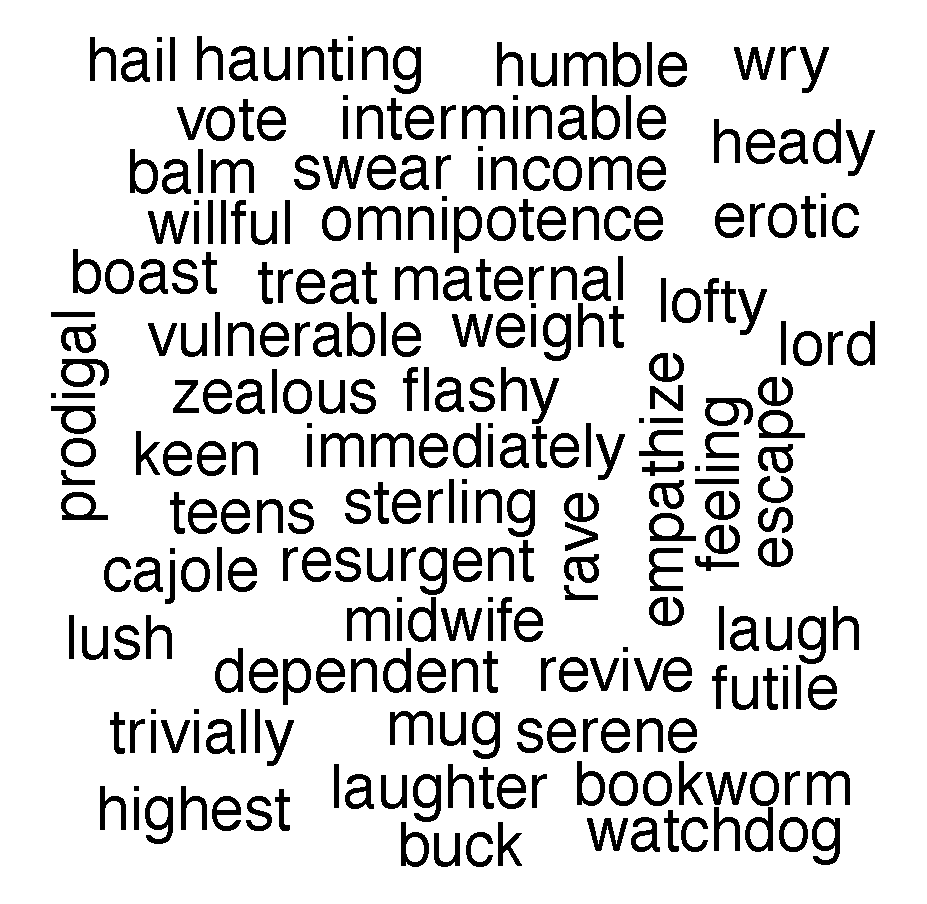
\includegraphics[scale=0.3]{clashes.pdf}
	\caption{Polarity clashes}
	\label{fig:word_clash}
\end{figure}


This high number of clashes found among different hand-made lexicons indicates two things: 1) Different human annotators can disagree when tagging a word to polarity classes. 2) There are several words that can belong to more than one sentiment class.  
Due to this, we can say that word-level polarity classification is a hard and subjective problem.  



% POS tags are not provided

\section{Obtaining labelled tweets}\label{sec:tweetlab}

In order to calculate our word-level time-series, we require a collection of time-stamped tweets with their corresponding polarity labels. 

We rely on the emoticon-based annotation approach in which tweets exhibiting positive :) and negative :( emoticons are labelled according to the emoticon's polarity \cite{go2010}. Afterwards, the emoticon used to label the passage is removed from the content.

% A limitation of this approach is its inability to capture neutral tweets. 
%The second approach applies a consensus of existing tweet classification methods. It considers tweets labelled to classes positive, negative, and neutral using two different methods: Sentiment140 and SentiStrength. All tweets where the two methods disagree are discarded.  

%Sentiment140\footnote{\url{http://www.sentiment140.com/}} is a Web application that classifies tweets using a maximum entropy classifier \cite{go2010} trained from a corpus of tweets labelled with the emoticon-based annotation approach. SentiStrength is a lexicon-based sentiment evaluator focused on social media messages written in English \cite{ThelwallBP12}. SentiStrength relies on a polarity lexicon, a negating word list, and an emoticon list, among other attributes, to analyse the content. The method returns a positive score, a negative score, and a polarity class with values positive, negative, and neutral.

Several researchers claim that general purpose lexical resources cannot reflect domain-specific language usage \cite{Choi2009, Zhou2014}. This means that the word polarities of the expanded lexicon will reflect the domains found in the collection from which the lexicon is built.  In this work, with the aim of creating general purpose lexicons, we consider two  collections of tweets covering multiple topics: The Edinburgh corpus (ED) \cite{Petrovic2010}, and the Stanford Sentiment corpus (STS) \cite{go2010}. These collections were gathered from  two Twitter APIs: the streaming API\footnote{\url{https://dev.twitter.com/streaming/overview}}, from which a real time sample of public posts can be retrieved, and the search API\footnote{\url{https://dev.twitter.com/rest/public/search}}, which allows the submission of queries composed by key-terms.

The ED corpus has 97 million tweets which were collected using the Twitter streaming API from a period spanning November 11th 2009 until February 1st 2010. This collection includes tweets in multiple languages. As was done in \cite{bifet2010}, non-English tweets were filtered out, and tweets exhibiting positive or negative emoticons were annotated using the emoticon-based approach. The remaining tweets were discarded.

The STS corpus was created by periodically sending queries :) and :( to the Twitter REST API between April 6th 2009 to June 25th 2009. All the tweets in this collection are written in English. The collection was labelled using the emotion-based annotation approach.

%The CON corpus was gathered by periocally sending queries to the Twitter REST API from 12th April to 22nd July 2012 regarding multiple topics. A parameter was specified to retrieve tweets written only in English. The topics were chosen from different domains that are frequently discussed in Twitter: politicians, countries, companies and long-standing topics. For the case of politicians, the studied period coincided with the electoral campaign of the U.S. 2012 presidential elections. We retrieved tweets related to both Republican and Democrat candidates Mitt Romney and Barack Obama. Additionally, we
%tracked tweets on the U.K prime minister David Cameron and the U.S. Democrat politician Hillary Clinton. We selected countries which face either an internal or external conflict situation: Iran, Israel and North Korea. We also tracked tweets related to two of the most influential high-tech companies in the world: Google and Facebook.  Finally, we selected two long-standing topics that are constantly discussed by the public: abortion and global warning. The total number of tweets in the collection is $5,175,984$. All these tweets were classified using Sentiment140 and SentiStrength and labelled using the consensus of methods. Hence, that all tweets were the two methods assigned a different class were discarded.



\begin{table}[htbp]
\begin{center}
\begin{tabular}{l|c|c}
\hline
 & ED & STS \\ \hline
Positive & $1,813,705$ & $800,000$  \\ 
Negative & $324,917$ & $800,000$  \\ \hline
Total & $2,138,622$ & $1,600,000$ \\ 
\end{tabular}
\end{center}
\caption{Collection statistics}
\label{tab:colstats}
\end{table}


The number of tweets for each polarity class in the two corpora is given in Table~\ref{tab:colstats}. We can observe that when using the streaming API (ED) positive emoticons occur much more frequently than negative ones.


\section{Word-level features}\label{sec:feat}

The word-level features proposed in this work exploit the temporal structure of a collection of polarity-labelled tweets. All the tweets from the collection are lowercased, tokenised and POS-tagged. We use the TwitterNLP library \cite{twitterNLP} that provides a  tokeniser and a tagger specific for the language used in Twitter. The tagger includes  nominal words classes, open and closed word classes, and Twitter specific classes such as hashtags, user mentions and emoticons. We prepend a POS-tag prefix to each word in order to differentiate homographs exhibiting different POS-tags.

We  treat the time-sorted collection of tweets as a data stream and create two types of time-series for each POS-tagged word observed in the vocabulary: the SGD series, and the SO series.

The first time-series is calculated by incrementally training a linear support vector machine using a stochastic gradient descent (SGD) online learning process \cite{Zhang2004}. The weights of this linear model correspond to POS-tagged words that are updated in an incremental fashion. We  optimise the hinge loss function with an $L_2$ penalty and a learning rate equal to $0.1$:
 
\begin{equation}\label{eq:sgd}
\frac{\lambda}{2}||w||^2+\sum [1- y (\mathbf{xw} +b) ]_{+}.
\end{equation}

The variables $\mathbf{w}$, $b$, and $\lambda$ correspond to the weight vector, the bias, and the regularisation parameter, respectively. The class labels $y$ are assumed to be in $\{+1,-1\}$, corresponding to positively and negatively labelled tweets, respectively. The regularisation parameter was set to $0.0001$.  As was suggested in \cite{bifet2010}, the model's weights determine how strongly the absence or presence of a word influences the prediction of negative and positive classes.  The SGD time-series is created by applying this learning process to a collection of labelled tweets and storing the word's coefficients in different time windows. We use time windows of $1,000$ examples.  

The second time-series corresponds to the accumulated semantic orientation (SO) introduced in Section~\ref{sec:related}. Let \emph{count} be a function that counts the number of times that a word or a sentiment label has been observed during a certain period of time. We calculate the SO score for each POS-tagged word in an accumulated way according to the following expression:   

\begin{equation}\label{eq:so}
 \operatorname{SO}(word) = log_2 \left( \frac{\operatorname{count}(\text{word $\wedge$ pos}) \times \operatorname{count}(\text{neg})}{\operatorname{count}(\text{word $\wedge$ neg}) \times \operatorname{count}(\text{pos})}\right)
\end{equation}


We use time windows of $1,000$ examples and the Laplace correction to avoid the zero-frequency problem. 


\begin{table}[htbp]
\footnotesize
\begin{center}
\begin{tabular}{l|l}
\hline
Feature & Description \\ \hline
mean &  The mean of the time-series. \\ 
trunc.mean &  The truncated mean of the time-series. \\ 
median &  The median of the time-series \\ 
last.element &  The last observation of the time-series.\\ 
sd &  The standard deviation of the time-series . \\ 
iqr &  The inter-quartile range. \\ 
sg &  The fraction of times the time-series changes its sign. \\ 
sg.diff &  The sg value for the  differenced time-series. \\ \hline
\end{tabular}
\end{center}
\caption{Time-series features}
\label{tab:feat}
\end{table}

We create SGD and SO time-series for positive and negative labelled tweets in our two datasets: ED, and STS. We refer to these time-series as \textbf{sgd.posneg} and \textbf{so.posneg}. 


We rely on our time-series to extract features which are used to train our world-level polarity classifier. These features intend to summarise properties of location and dispersion of the time-series and are listed in Table~\ref{tab:feat}. Location-oriented features \emph{mean}, \emph{trimm.mean} and \emph{median} measure the central tendency of the time-series. The feature \emph{last.element} corresponds to the last value observed in the time-series.  This attribute  would be equivalent to the traditional SO measure for the so.posneg time-series. The features \emph{sd}, \emph{iqr}, \emph{sg}, and \emph{sg.diff} intend to measure the level of dispersion of the time-series. 

In addition to these time-series features, we include the POS-tag of the word as a nominal attribute.



\section{Experiments}\label{sec:lex_expand}

In this section, we present our experimental results for Twitter lexicon expansion. In the first part, we study the word-level polarity classification problem. In the second part, we expand the lexicon using the trained classifier and use it for message-level  polarity classification of tweets. 

\subsection{Word-level polarity classification}

We calculated the time-series described in Section~\ref{sec:feat} for the most frequent $10,000$ POS-tagged words found in each of our two datasets. The time-series were calculated using MOA\footnote{\url{http://moa.cs.waikato.ac.nz/}}, a data stream mining framework. The resulting time-series \textbf{sgd.posneg} and \textbf{so.posneg} for a sample of words in the STS dataset are shown in Figure~\ref{fig:timeseries}. 

\begin{figure}[htb]
\begin{center}
\begin{tabular}{c}
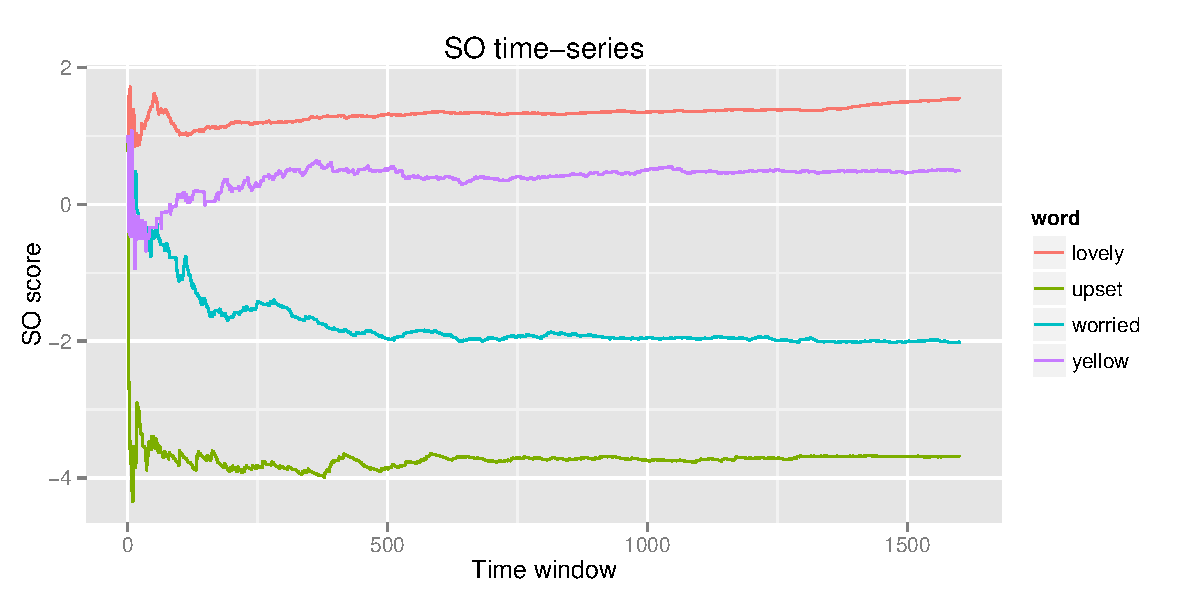
\includegraphics[scale=0.45]{SOseries.pdf} \\
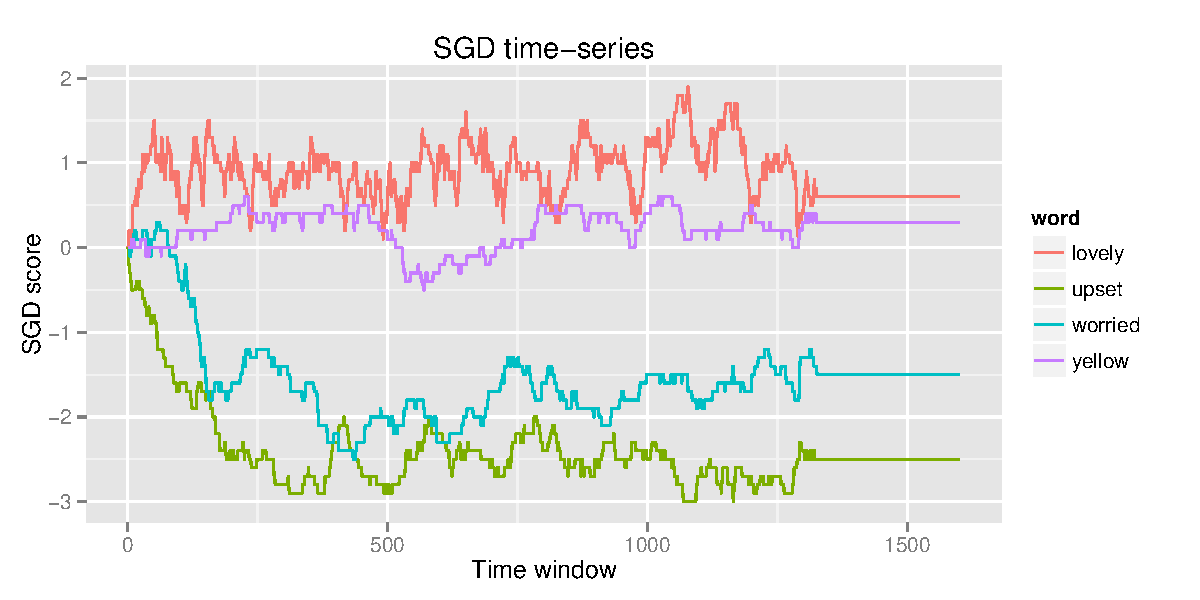
\includegraphics[scale=0.45]{SGDseries.pdf}\\
\end{tabular}
\caption{Word-level time-series.}
\label{fig:timeseries}
\end{center}
\end{figure}


\begin{table}[htb]
\begin{center}
\begin{tabular}{l|c|c}
\hline
 & ED & STS \\ \hline
Positive & 1027 & 1023 \\ 
Negative & 806 & 985 \\ 
Neutral & 1814 & 1912 \\ 
Total & 3647 & 3920 \\ \hline
\end{tabular}
\end{center}
\caption{Word-level polarity classification datasets.}
\label{tab:wordcorpus}
\end{table}


We can observe that the positive and neutral words \emph{lovely} and \emph{yellow} exhibit greater SO and SGD scores than the negative words  \emph{worried} and \emph{upset}. This  suggests a correspondence between time-series values and the word's polarities. However, we can see that the SO time-series are much more stable than the SGD ones. We believe that SO is more stable than SGD because, as shown in Equation~\ref{eq:so}, SO treats words  independently from each other given the sentiment class. On the other hand, SGD scores are updated according to the SGD learning rule, which comes from the sub-gradient of Equation~\ref{eq:sgd}. In this rule, the coefficients are updated every time the learning SVM misclassifies an example from the stream of emoticon-labelled tweets ($y(\mathbf{xw} +b) <1$). Therefore, the change of the weight of a particular word depends both on the sentiment label, and the co-occurring words within the tweets from the training collection.  


To create training and test data for machine learning, all the POS-tagged words matching the metalexicon are labelled according to the lexicon's polarities. It is interesting to consider how frequently positive, negative, and neutral words occur in a collection of tweets. The number of words labelled as positive, negative, and neutral for both the ED and STS datasets is given in Table~\ref{tab:wordcorpus}. As shown in the table, neutral words are the most frequent words in both datasets. Moreover, positive words are more frequent than the negative ones. 



As the lexicon's entries are not POS-tagged, we assume that all posible POS-tags of a word have the same polarity. However, this assumption can introduce noise in the training data. For example, the word \emph{ill}, which is labelled as negative by the lexicon, will be labelled as negative for two different POS-tags: adjective, and nominal+verbal contraction. This word is very likely to express a negative sentiment when used as an adjective, but it is unlikely to express a negative sentiment when it refers in a misspelled way to the contraction \emph{I'll}. A simple outlier removal technique to deal with this problem will be discussed in Section~\ref{sec:messlevel}.
 

   
Once our time-series are created, we extract from them the word-level features described in Section~\ref{sec:feat}. The feature values obtained for the words used in the time-series visualisation example (Figure~\ref{fig:timeseries}) are given in Table~\ref{fig:featex}.  We can see that each entry has a POS-tag prefix.  As expected, location-oriented features from the same time-series exhibit similar values. %Considering that we have several highly mutually correlated features, we will have to avoid using learning algorithms that are sensitive to this type of data.

\begin{table}[htb]
\scriptsize
\centering
\begin{tabular}{l|llll}
  \hline
Attribute & A-lovely & A-yellow & A-upset & V-worried \\ 
  \hline
sgd.last &  0.6 &  0.3 & -2.5 & -1.5 \\ 
  sgd.mean &  0.9 &  0.2 & -2.4 & -1.6 \\ 
  sgd.trimm.mean &  0.9 &  0.2 & -2.5 & -1.6 \\ 
  sgd.median &  0.9 &  0.3 & -2.5 & -1.6 \\ 
  sgd.sd & 0.3 & 0.2 & 0.5 & 0.5 \\ 
  sgd.sg & 0.0 & 0.0 & 0.0 & 0.0 \\ 
  sgd.sg.diff & 0.2 & 0.0 & 0.1 & 0.0 \\ 
  sgd.iqr & 0.5 & 0.3 & 0.3 & 0.3 \\ 
  so.last &  1.5 &  0.5 & -3.7 & -2.0 \\ 
  so.mean &  1.3 &  0.4 & -3.7 & -1.8 \\ 
  so.trimm.mean &  1.3 &  0.4 & -3.7 & -1.9 \\ 
  so.median &  1.3 &  0.5 & -3.7 & -1.9 \\ 
  so.sd & 0.1 & 0.2 & 0.2 & 0.4 \\ 
  so.sg & 0.0 & 0.0 & 0.0& 0.0 \\ 
  so.sg.diff & 0.5 & 0.4 & 0.4 & 0.4 \\ 
  so.iqr & 0.1 & 0.1 & 0.1 & 0.1 \\ 
  pos.tag & adjective & adjective & adjective & verb \\ \hline
  label & positive & neutral & negative & negative \\ 
   \hline
\end{tabular}
\caption{Word-level feature example.}
\label{fig:featex}
\end{table}



A scatterplot between attributes \textbf{sgd.mean} and \textbf{so.mean} for the labelled words from the STS corpus is shown in Figure~\ref{fig:sosgd}. From the figure we can observe that both variables are highly correlated. The correlation is 0.858 and 0.877 for the ED and STS corpora respectively. Positive, negative, and neutral words are depicted with different colours. We can observe that negative words tend to show low values of sgd.mean and so.mean, and positive words tend to show the opposite. Neutral words are more spread out and hard to distinguish.  This pattern can also be clearly seen in the boxplots shown in Figure~\ref{fig:box}. We can observe from the boxplots that the three classes of words can exhibit different densities in both variables sgd.mean and so.mean. The medians of the classes show an accurate correspondence with the word's polarity, i.e., $\operatorname{median}(pos) > \operatorname{median}(neu) > \operatorname{median}(neg)$. The boxplots also show a substantial number of outliers, especially for neutral words. 


\begin{figure}[htb]
	\centering
	 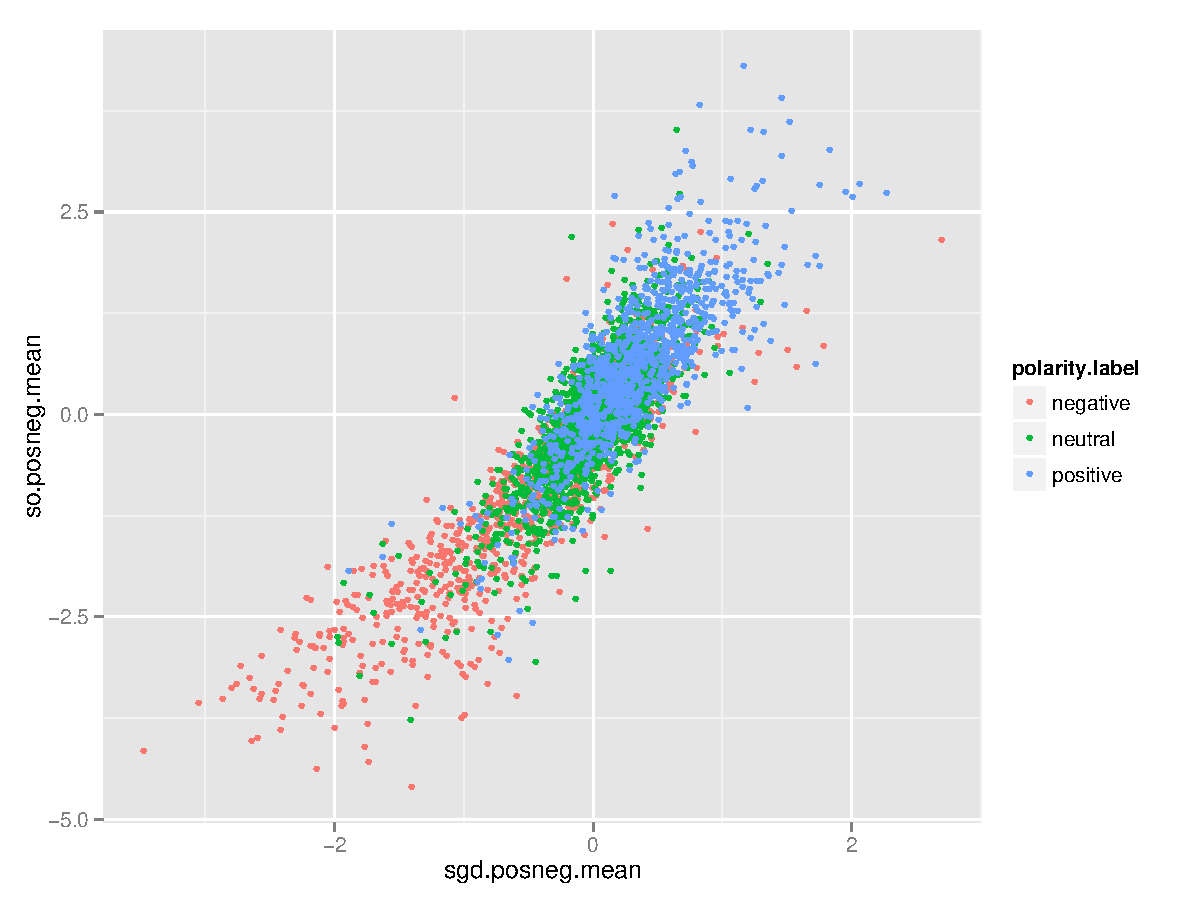
\includegraphics[width=7.5cm,height=6cm]{SGDSO.pdf}
	\caption{SO vs SGD scatterplot.}
	\label{fig:sosgd}
\end{figure}



\begin{figure}[ht]
\begin{center}
\begin{tabular}{c}
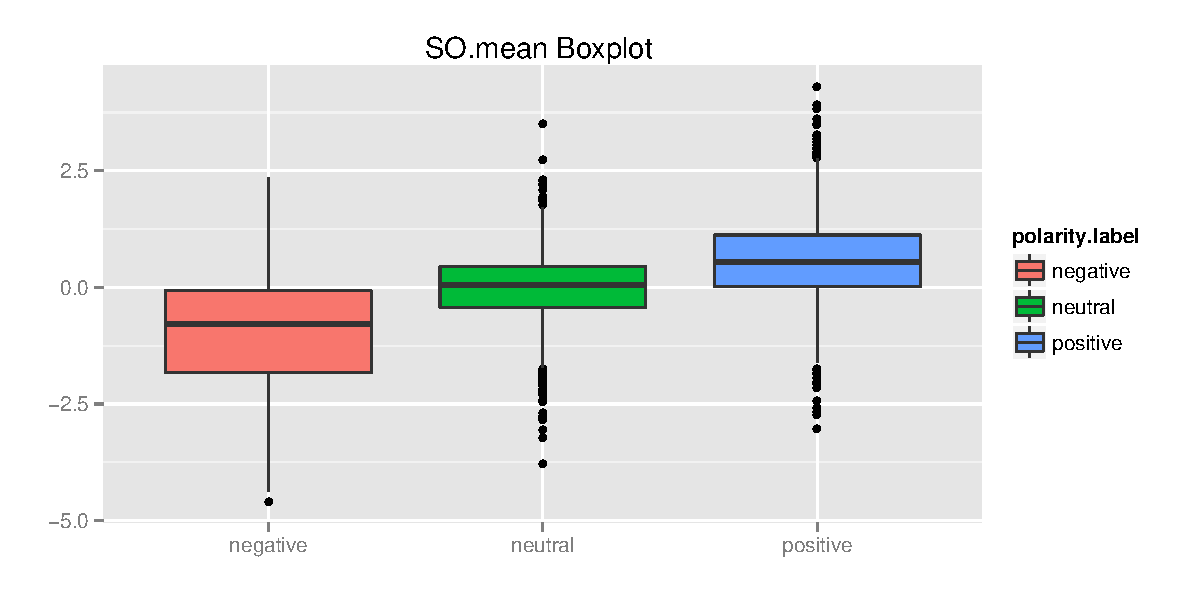
\includegraphics[scale=0.45]{SObox.pdf}\\
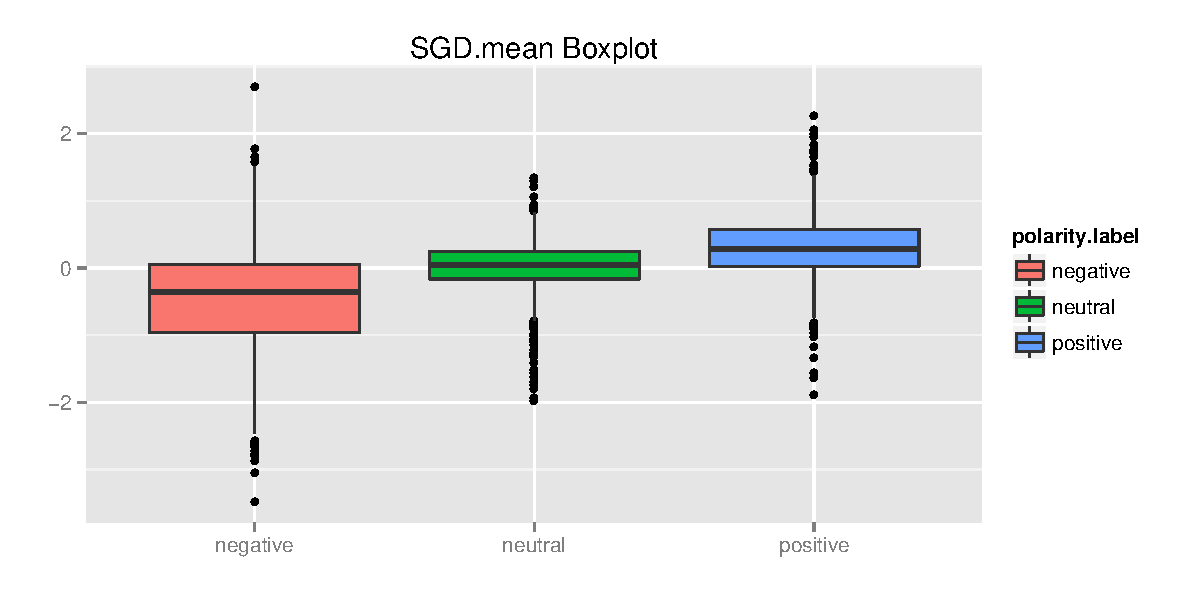
\includegraphics[scale=0.45]{SGDbox.pdf}
\end{tabular}
\caption{SO and SGD  Boxplots.}
\label{fig:box}
\end{center}
\end{figure} 

 
Next, we focus on the word-level classification problem. With the aim of gaining a better understanding of the problem, we study three word-level classification problems:
\begin{enumerate}
\item  \emph{Neutrality}: Classify words as neutral (objective) or non-neutral (subjective). We label positive and negative words as non-neutral for this task.
\item \emph{PosNeg}: Classify words to positive or negative classes. We remove all neutral words for this task. 
\item \emph{Polarity}: Classify words to classes positive, negative or neutral. This is the classification problem we aim to solve. 
\end{enumerate}

We study the information provided by each feature with respect to the three classification tasks described above. This is done by calculating the information gain of each feature. This score is normally used for decision tree learning and  measures the reduction of entropy within each class after performing the best split induced by the feature. The information gains obtained for the different attributes in relation to the three classification tasks are shown in Table~\ref{tab:infogains}.
 
\begin{table*}[htb]
\footnotesize
\centering
\begin{tabular}{l|ccc|ccc}
\hline
Dataset & \multicolumn{3}{c|}{ED} & \multicolumn{3}{c}{STS} \\ \hline
 Task &  Neutrality & PosNeg & Polarity &  Neutrality & PosNeg & Polarity  \\ \hline
pos-tag &  0.062 & 0.017  & 0.071 & 0.068 & 0.016 & 0.076  \\ 
sgd.mean & \textbf{0.082}  & 0.233  &  0.200 & \textbf{0.104} & 0.276 & \textbf{0.246}  \\ 
sgd.trimm.mean & 0.079 & 0.237 & 0.201 & \textbf{0.104} & 0.276 & 0.242 \\ 
sgd.median & 0.075 & 0.233 & 0.193  & 0.097 & 0.275 & 0.239 \\ 
sgd.last & 0.057 & 0.177 & 0.155  & 0.086 & 0.258 & 0.221  \\ 
sgd.sd & 0.020 & 0.038 & 0.034  & 0.030 & 0.030 & 0.052 \\
sgd.sg & 0.029 & 0.000 & 0.030 & 0.049 & 0.017 & 0.062 \\
sgd.sg.diff &  0.000 & 0.000 & 0.008 & 0.005 & 0.000 & 0.000 \\ 
sgd.iqr &  0.018 & 0.012 & 0.019 & 0.015 & 0.014 & 0.017 \\ 
so.mean & 0.079 & 0.283 & \textbf{0.219}  & 0.081 & \textbf{0.301} & 0.232 \\ 
so.trimm.mean & 0.077 & \textbf{0.284} & 0.215 & 0.079 & 0.300 & 0.229 \\ 
so.median & 0.077 & 0.281 & 0.215 & 0.076 & 0.300 & 0.228 \\
so.last & 0.069 & 0.279  &  0.211 & 0.084 & 0.300 & 0.240  \\  
so.sd  & 0.000 & 0.015 & 0.008 & 0.000 & 0.012 & 0.007 \\
so.sg &  0.013 & 0.216 & 0.126 & 0.019 & 0.239 & 0.142 \\ 
so.sg.diff & 0.000 & 0.012 & 0.009 & 0.000 & 0.000 & 0.000 \\
so.iqr & 0.000 & 0.000 & 0.000  & 0.000 & 0.008 & 0.000 \\      \hline
\end{tabular}
\caption{Information gain values.}
\label{tab:infogains}
\end{table*}
 


We can observe that variables measuring the location of the SO and SGD time-series tend to be more informative than the ones measuring dispersion. Moreover, the information gain of these variables is much higher for PosNeg than for neutrality. SGD and SO are competitive measures for neutrality, but SO is far better for PosNeg. An interesting insight is that features that measure the central tendency of the time-series tend to be more informative than the last values, especially for SGD. These measures smooth the fluctuations of the SGD time-series. We can see that the feature \emph{sgd.mean} is the best attribute for neutrality classification in both datasets. We can also see that POS tags are useful for neutrality detection, but useless for PosNeg. Therefore, we can conclude that positive and negative words have a similar distribution of POS tags. 

We trained supervised classifiers for the three different classification problems in both datasets STS and ED. The classification experiments were performed using WEKA\footnote{\url{http://www.cs.waikato.ac.nz/ml/weka/}}, a machine learning environment. We studied the following learning algorithms in some preliminary experiments: RBF SVM, Logistic regression, C4.5, and Random Forest. As the RBF SVM produced the best performance among the different methods, we used this method in our  classification experiments with a nested grid search procedure for parameter tuning. 

The evaluation was done using 10 times 10-folds-cross-validation and different sub-sets of attributes were compared.  All the methods are compared with the baseline of using the last value of the semantic orientation, based on a corrected paired t-student test with an alpha level of $0.05$ \cite{nadeau2003inference}.  We used the following  sub-sets of attributes: 1) \emph{SO}: Includes only the feature \emph{so.last}. This is the baseline and is equivalent to the standard semantic orientation measure with the decision boundaries provided by the SVM. 2) \emph{ALL}: Includes all the features. 3)\emph{SGD.TS+POS}: Includes all the SGD-oriented features and the POS tag. 4)\emph{SO+POS}: Includes the features \emph{so.last} and the POS tag.

We evaluate the classification accuracy and the weighted area under the ROC curves (AUCs) (to deal with class imbalances) for the four different sub-sets of attributes in the two datasets.  The classification results are presented in Table~\ref{tab:classres}. The symbols $\circ$ and $\bullet$ correspond to statistically significant improvements and degradations with respect to the baseline, respectively.

We can observe a much lower performance in Neutrality detection than in PosNeg. This validates the hypothesis that the detection of neutral Twitter words is much more harder than distinguishing between positive and negative words.  
The performances between both datasets tends to be similar. However, the AUC results in STS are better than in ED. This suggests that a collection of balanced positive and negative labelled tweets could be more suitable for lexicon expansion. 
Another important result, is that the combination of all features leads to a significant improvement over the baseline in accuracy and AUC for neutrality and polarity classification. In the PosNeg classification task we can see that the baseline is very strong. This suggests that SO is very good for discriminating between positive and negative words, but not strong enough when neutral words are included.
Regarding SO and SGD time-series, we can conclude that they are competitive for neutrality detection. However, SO-based features are better for PosNeg and Polarity tasks. 

\begin{table*}[!htb]
\begin{center}
\begin{tabular}{l|l|l|l|l|l}
\hline \hline
\multicolumn{ 6}{c}{Accuracy } \\ \hline \hline
Dataset & SO & ALL & SGD.TS+POS & SO.TS+POS & SO+POS \\ \hline
ED-Neutrality & 61.52 $\pm$ 2.21 & \textbf{65.16 $\pm$ 2.09} $\circ$ & 64.55 $\pm$ 2.27 $\circ$ & 64.9 $\pm$ 2.14  $\circ$ & 64.18 $\pm$ 2.12 $\circ$ \\ 
ED-PosNeg & 74.78 $\pm$ 2.93 & \textbf{76.04 $\pm$ 2.72} & 73.61 $\pm$ 2.51 & 75.6 $\pm$ 2.84 & 74.99 $\pm$ 2.72 \\ 
ED-Polarity & 59.48 $\pm$ 2.29 & \textbf{61.93 $\pm$ 2.1 $\circ$} & 60.97 $\pm$ 1.96 & 61.73 $\pm$ 1.98 $\circ$ & 61.57 $\pm$ 2.04 $\circ$ \\  \hline
STS-Neutrality & 62.99 $\pm$ 2.03 & \textbf{66.2 $\pm$ 2.11 $\circ$} & 65.26 $\pm$ 2.34 $\circ$ & 65.73 $\pm$ 1.98 $\circ$ & 65.77 $\pm$ 2.09 $\circ$ \\ 
STS-PosNeg & \textbf{77.18 $\pm$ 2.88} & 76.98 $\pm$ 2.82 & 75.39 $\pm$ 2.89 $\bullet$ & 76.76 $\pm$ 2.89 & 76.98 $\pm$ 2.71 \\ 
STS-Polarity & 60.2 $\pm$ 2.23 & \textbf{62.74 $\pm$ 1.52} $\circ$ & 62.34 $\pm$ 1.61 $\circ$ & 62.14 $\pm$ 1.73 $\circ$ & 62.1 $\pm$ 1.78 $\circ$ \\  \hline \hline
\multicolumn{ 6}{c}{Weighted AUC } \\ \hline \hline
Dataset & SO & ALL & SGD.TS+POS & SO.TS+POS & SO+POS \\ \hline
ED-Neutrality & 0.62 $\pm$ 0.02 &  \textbf{0.65 $\pm$ 0.02} $\circ$ & \textbf{0.65 $\pm$ 0.02} $\circ$  & \textbf{0.65 $\pm$ 0.02} $\circ$ & 0.64 $\pm$ 0.02 $\circ$ \\ 
ED-PosNeg & 0.74 $\pm$ 0.03 & \textbf{0.75 $\pm$ 0.03} & 0.71 $\pm$ 0.03 $\bullet$ & 0.74 $\pm$ 0.03 & 0.73 $\pm$ 0.03 \\ 
ED-Polarity & 0.62 $\pm$ 0.02 &  \textbf{0.65 $\pm$0.02} $\circ$ & 0.64 $\pm$ 0.02 & \textbf{0.65 $\pm$ 0.02} $\circ$ & 0.64 $\pm$ 0.02 $\circ$ \\ \hline
STS-Neutrality & 0.63 $\pm$ 0.02 & \textbf{0.67 $\pm$ 0.02} $\circ$             & 0.66 $\pm$ 0.02 $\circ$  & 0.66 $\pm$ 0.02 $\circ$ & 0.66 $\pm$ 0.02$\circ$ \\ 
STS-PosNeg & \textbf{0.77 $\pm$ 0.03} &  \textbf{0.77 $\pm$ 0.03} & 0.75 $\pm$ 0.03 $\bullet$ & \textbf{0.77 $\pm$ 0.03} & \textbf{0.77 $\pm$ 0.03} \\ 
STS-Polarity & 0.64 $\pm$ 0.02 & \textbf{0.66 $\pm$ 0.01} $\circ$  & 0.65 $\pm$ 0.02 $\bullet$  & \textbf{0.66 $\pm$ 0.02} $\circ$ & \textbf{0.66 $\pm$ 0.02} $\circ$ \\ \hline 
\end{tabular}
\end{center}
\caption{World-level classification performance.} 
\label{tab:classres}
\end{table*}



\subsection{Lexicon expansion}\label{sec:messlevel}
The ultimate goal of the polarity-classification of words is to produce a Twitter-oriented opinion lexicon based on the properties of SentiWordet, i.e., a lexicon of POS-tagged disambiguated entries with their corresponding distribution for positive, negative, and neutral classes.  To do this, we fit a logistic regression model to the outputs of the support vector machine trained for the \emph{polarity} problem using all the attributes. 
The resulting model is then used to classify the remaining unlabelled words. This process is performed for both STS and ED datasets.

A sample from the expanded word list is given in Table~\ref{tab:expwords}. We can see that each entry has the following attributes: the word, the POS-tag, the sentiment label that corresponds to the class with maximum probability, and the distribution. We inspected the expanded lexicon and observed that the estimated probabilities tend to agree with the desired values. However, there are some words for which the estimated distribution makes no sense at all, such as the word \emph{same} from the example.


\begin{table}[htbp]
\scriptsize
\begin{tabular}{l|l|l|r|r|r}
\hline
word & POS & label & negative & neutral& positive \\ \hline
alrighty & interjection & positive & 0.021 & 0.087 & 0.892 \\ 
boooooo & interjection & negative & 0.984 & 0.013 & 0.003 \\ 
lmaoo & interjection & positive & 0.19 & 0.338 & 0.472 \\ 
french & adjective & neutral & 0.357 & 0.358 & 0.285 \\ 
handsome & adjective & positive & 0.007 & 0.026 & 0.968 \\ 
saddest & adjective & negative & 0.998 & 0.002 & 0 \\ 
same & adjective & negative & 0.604 & 0.195 & 0.201 \\ 
anniversary & common.noun & neutral & 0.074 & 0.586 & 0.339 \\ 
tear & common.noun & negative & 0.833 & 0.124 & 0.044 \\ 
relaxing & verb & positive & 0.064 & 0.244 & 0.692 \\ 
wikipedia & proper.noun & neutral & 0.102 & 0.644 & 0.254 \\ \hline
\end{tabular}
\caption{Expanded words example.}
\label{tab:expwords}
\end{table}

The provided probabilities can also be used to explore the sentiment intensities of words. In Figure~\ref{fig:wordcloud}, we visualise the expanded lexicon intensities of words classified as positive and negative through word clouds. The sizes of the words are proportional to the log odds ratios $\log_2(\frac{P(pos)}{P(neg)})$ and $\log_2(\frac{P(neg)}{P(pos)})$ for positive and negative words, respectively. 


\begin{figure}[ht]
\begin{center}
\begin{tabular}{cc}
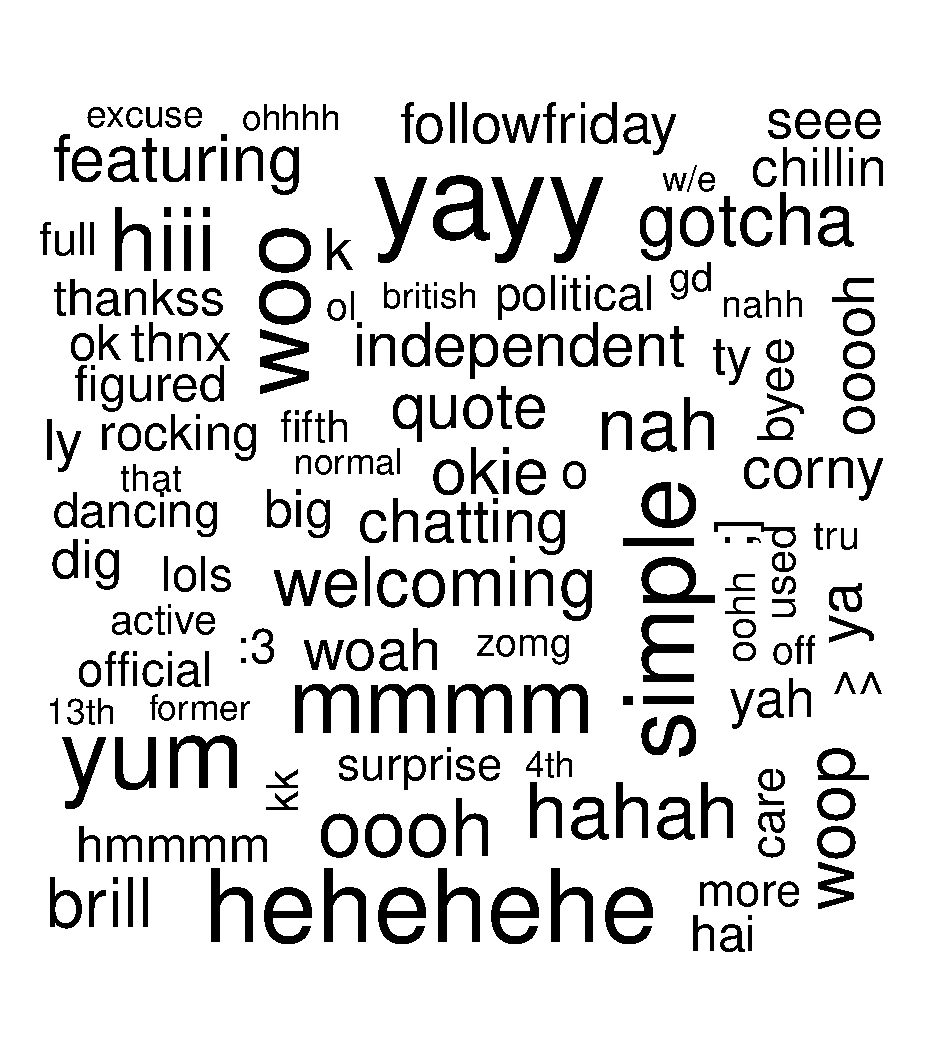
\includegraphics[scale=0.25]{poswords.pdf}
&
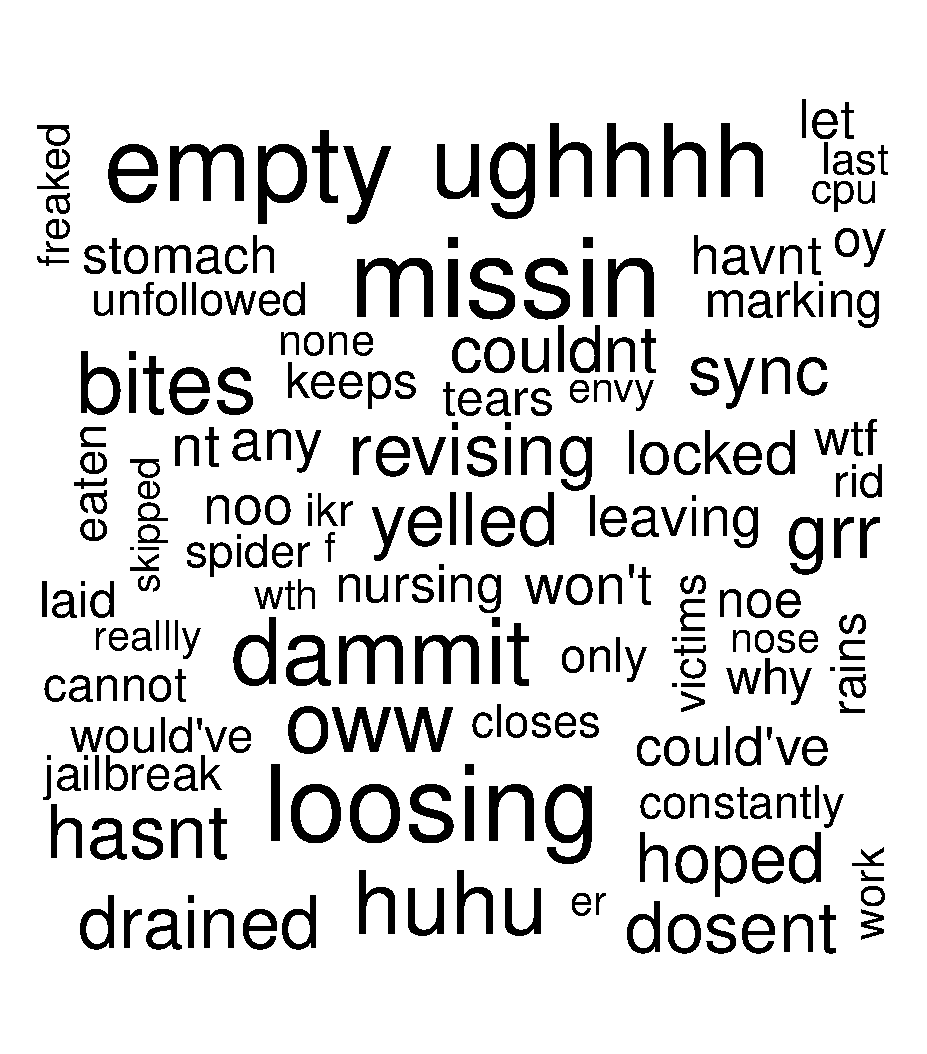
\includegraphics[scale=0.25]{negwords.pdf}\\
(a) & (b)  
\end{tabular}
\caption{Word clouds of positive and negative words using log odds proportions.}
\label{fig:wordcloud}
\end{center}
\end{figure}



Next, we study the usefulness of our expanded lexicons ED and STS for Twitter polarity classification. This involves categorising a whole tweet according to positive or negative sentiment classes. Lexicon-based methods have shown to be more effective in distinguishing positive and negative messages than for the detection of subjectivity \cite{BravoMarquez2014}. Therefore, we omit the detection of neutral tweets. The experiments are performed on three collections of tweets that were manually annotated to positive and negative classes. The first collection is  \emph{6HumanCoded}\footnote{\url{http://sentistrength.wlv.ac.uk/documentation/6humanCodedDataSets.zip}}, which was used to evaluate SentiStrength \cite{ThelwallBP12}.  In this dataset tweets are scored according to a positive and negative numerical scores. We use the difference of these scores to create polarity classes and discard messages where this difference is equal to zero. The other datasets are   \emph{Sanders}\footnote{\url{http://www.sananalytics.com/lab/twitter-sentiment/}}, and \emph{SemEval}\footnote{\url{http://www.cs.york.ac.uk/semeval-2013/task2/}}. The number of positive and negative words per corpus is given in Table~\ref{tab:polcorpus}.
  
 \begin{table}[htbp]
\begin{center}
\begin{tabular}{l|c|c|c}
\hline
 & Positive & Negative & Total \\ \hline
6Coded & 1340 & 949 & 2289 \\ 
Sanders & 570 & 654 & 1224 \\ 
SemEval & 5232 & 2067 & 7299 \\ \hline
\end{tabular}
\end{center}
\caption{Message-level polarity classification datasets.}
\label{tab:polcorpus}
\end{table} 
  
\begin{table*}[htbp]
\begin{center}
\begin{tabular}{l|l|l|l|l}
\hline \hline
\multicolumn{ 5}{c}{Accuracy } \\ \hline \hline
Dataset & Baseline & ED & STS & Combination \\ \hline
6-coded & 71.79 $\pm$ 2.79 & 74.91 $\pm$ 2.56 $\circ$ & 75.11 $\pm$ 2.66 $\circ$ &  \textbf{75.31 $\pm$ 2.42} $\circ$ \\ 
Sanders & 71.43 $\pm$ 3.76 & 77.17 $\pm$ 3.68 $\circ$ & 77.32 $\pm$ 4.09 $\circ$ &  \textbf{77.54 $\pm$ 3.64} $\circ$ \\ 
SemEval & 76.81 $\pm$ 1.22 & 76.66 $\pm$ 1.38 & 77.7 $\pm$ 1.25 $\circ$ & \textbf{78.13 $\pm$ 1.38} $\circ$ \\ \hline \hline
\multicolumn{ 5}{c}{Weighted AUC } \\ \hline \hline
Dataset & Baseline & ED & S140 & Combination \\ \hline
6-coded & 0.77 $\pm$ 0.03 & 0.82 $\pm$ 0.03 $\circ$ & 0.82 $\pm$ 0.02 $\circ$ &  \textbf{0.83 $\pm$ 0.02} $\circ$ \\ 
Sanders & 0.77 $\pm$ 0.04 & 0.83 $\pm$ 0.04 $\circ$ & \textbf{0.84 $\pm$ 0.04} $\circ$  & \textbf{0.84 $\pm$ 0.04} $\circ$ \\ 
SemEval & 0.77 $\pm$ 0.02 & 0.81 $\pm$ 0.02 $\circ$ & \textbf{0.83 $\pm$ 0.02} $\circ$ &  \textbf{0.83 $\pm$ 0.02} $\circ$ \\ \hline
\end{tabular}
\caption{Message-level polarity classification performance.}
\label{tab:messclass}
\end{center}
\end{table*}


\begin{table*}[htbp]
\begin{center}
\begin{tabular}{l|l|l|l|l}
\hline
\hline
\multicolumn{5}{c}{Accuracy } \\ \hline \hline
Dataset & Baseline & ED & S140 &  Combination \\ \hline
6Coded & 71.79 $\pm$ 2.79 & \textbf{ 76.57 $\pm$ 2.3} $\circ$ & 75.28 $\pm$ 2.5 $\circ$ & 76.52 $\pm$ 2.43 $\circ$ \\ 
Sanders & 71.43 $\pm$ 3.76 & 76.78 $\pm$ 3.99 $\circ$ & 75.83 $\pm$ 4.19 $\circ$  & \textbf{76.88 $\pm$ 4.06} $\circ$ \\ 
SemEval & 76.81 $\pm$ 1.22 & 78.23 $\pm$ 1.3 $\circ$ & 77.07 $\pm$ 1.18 & \textbf{78.35 $\pm$ 1.24} $\circ$ \\ \hline \hline
\multicolumn{ 5}{c}{Weighted AUC } \\ \hline \hline
Dataset & Baseline & ED & S140 & Combination \\ \hline 
6Coded & 0.77 $\pm$ 0.03 & \textbf{0.84 $\pm$ 0.02} $\circ$ & 0.82 $\pm$ 0.03 $\circ$ &  \textbf{0.84 $\pm$ 0.02} $\circ$ \\ 
Sanders & 0.77 $\pm$ 0.04 & \textbf{0.83 $\pm$ 0.04} $\circ$ & 0.82 $\pm$ 0.04 $\circ$ & \textbf{0.83 $\pm$ 0.04} $\circ$ \\ 
SemEval & 0.77 $\pm$ 0.02 & 0.83 $\pm$ 0.02 $\circ$ & 0.82 $\pm$ 0.02 $\circ$  & \textbf{0.84 $\pm$ 0.02} $\circ$ \\ \hline
\end{tabular}
\caption{Message-level polarity classification performance with outlier removal.}
\label{tab:messclassout}
\end{center}
\end{table*}



We train a logistic regression on the labelled collections of tweets  based on simple count-based features extracted using the lexicons. It is important to recall that our expanded lexicons do not include the training words from the metalexicon. Hence, there is no overlap between the metalexicon and the expanded lexicons. We compute features in the following manner. We count the number of positive and negative words from the metalexicon  matching the content of the tweet. From the expanded lexicons we create a positive and a negative score. The positive score is calculated by adding the positive probabilities of POS-tagged words labelled as positive within the tweet's content. The negative score is calculated in an analogous way from the negative probabilities. The neutral label provided by the expanded lexicons is used for discarding non-opinion words. 

We study four different setups based on these attributes. 1) \emph{Baseline}: It includes the attributes calculated from the metalexicon.  2) \emph{ED}: It includes the baseline and the attributes from the ED expanded lexicon. 3) \emph{STS}: This one is analogus to ED, but using the STS lexicon. 4) \emph{Combination}: It includes the baseline, ED, and STS.

In the same way as in the word-level classification task, we rely on the accuracy and the weighted AUC as evaluation measures, and we compare the different setups with the baseline using the corrected paired t-tests. The classification results obtained for the different setups are shown in Table~\ref{tab:messclass}.


The results indicate that the expanded lexicons produce meaningful improvements in performance over the baseline on the different datasets. The performance of STS is slightly better than ED. This pattern was also observed in the word-level classification performances shown in Table~\ref{tab:classres}. This suggests that the two different ways for evaluating the lexicon expansion, one at the word level and the other at the message level, are consistent with each other. When we rely on the AUC criterion the improvements become more significant on SemEval, which is the largest dataset. We can also observe that the best accuracies are obtained when the attributes from both expanded lexicons are used. Therefore, we can conclude that lexicons expanded from different collections of tweets complement each other to some extent.  



As was discussed in the previous section, the metalexicon does not provide POS-tagged entries. Therefore, words exhibiting  multiple POS-tags were labelled with the same polarity in the word-level training data. We also mentioned that this assumption could make the classifier learn spurious patterns and erroneously classify unlabelled words. For example the word \emph{ill} together with the POS-tag \emph{nominal+verb} receives a negative label. However, when \emph{ill} is used with this part of speech to refer to the contraction of the pronoun \emph{I} and the verb \emph{will}, it should be labelled as neutral instead. Moreover, by inspection we realised that \emph{ill} is the only labelled entry with the POS \emph{nominal+verb}. Considering that the POS tag is also used as a feature in the word-level classifiers, we observed that most of the words exhibiting the POS tag \emph{nominal+verb} in both expanded lexicons were classified to the negative class. Common sense suggests that these words should be expanded to the neutral class.

In order to avoid learning this type of spurious pattern, we re-trained the word-level classifiers using an outlier removal technique. More specifically, we clean out the instances from the word-level training data that are misclassified by a classifier trained using 10-folds cross-validation. Afterwards, we retrain the word-level classifiers and create new versions of the expanded lexicons for both STS and ED datasets. In the new versions of the expanded lexicons, words exhibiting the \emph{nominal+verb} POS are classified to the neutral class.

The message-level classification results obtained by the expanded lexicons with outlier removal are shown in Table~\ref{tab:messclassout}. There is improvement in performance for the ED lexicon for the \emph{6Coded} and \emph{Sanders} datasets in comparison to the results obtained by the original expanded lexicons. Apparently, the ED corpus is more susceptible to outliers than STS. Additionally, for the datasets \emph{6Coded} and \emph{Sanders} the best accuracies and AUC scores obtained with outlier-cleansed lexicons are better than the best performances obtained with the original lexicons as displayed in Table~\ref{tab:messclass}.


\section{Conclusions}\label{sec:conc}

In this article, we presented a supervised method for opinion lexicon expansion in the context of Twitter messages. The method creates a lexicon with disambiguated POS entries and a probability distribution for positive, negative, and neutral classes. 

To the best of our knowledge, this is the first approach for creating Twitter opinion lexicons with these characteristics. Considering that these characteristics are very similar to those of SentiWordNet, a well-known publicly available lexical resource, we believe that several sentiment analysis methods that are based on SentiWordnet can be easily adapted to Twitter by relying on our lexicon. The source-code of our method, together with  the expanded lexicons are publicly available to the research community\footnote{\url{https://github.com/felipebravom/TwitterSentLex}}.

Our supervised framework for lexicon expansion opens several directions for further research. 

The method could be used to create domain-specific lexicons by relying on tweets collected from the target domain. However, there are many domains such as politics, in which emoticons are not frequently used to express positive and negative opinions. New ways for automatically labelling collections of tweets should be explored. We could rely on other domain-specific expressions such as hashtags, or use message-level classifiers trained from domains in which emoticons are frequently used. 

Other types of word-level features based on the context of the word can be explored. We could rely on well-known opinion properties such as negations, opinion shifters, and intensifiers, to create these features.

Another important problem to be studied is how to reduce the noise of the seed lexicon. This could be addressed by manually cleaning the lexicon or by exploring different outlier removal techniques.

We believe that unlabelled words and their feature values could provide valuable information which is not being exploited so far. Semi-supervised methods such as the EM algorithm \cite{nigam2006semi} could be used to include unlabelled words as part of the training process. 

Recalling that our word-level features are based on time-series, they could be easily calculated in an on-line fashion from a stream of time-evolving tweets. Based on this, we could study the dynamics of opinion words. New opinion words could be discovered, as the change of the distribution in certain words could be tracked. This approach could be used for online lexicon expansion in specific domains, and potentially be useful for high impact events on Twitter, such as elections and sports competitions.


\bibliographystyle{abbrv}
\bibliography{bio}


\end{document}
